\documentclass[12pt]{article}
\usepackage{graphicx}
\usepackage{float}
\usepackage{hyperref}
\begin{document}
	\title{ECS 171 Group 2 - Predicting Housing Prices in Austin, Texas}
	\author{Jackson Gaydon et al (add the others before submitting)}
	\date{12/5/12} 
	\maketitle
	
	\section{Introduction and Background} 
	
	For many, buying a house will be their most expensive purchase. Not only that, but it will be the greatest share of their assets and will be their greatest accumulator of wealth. As such, it can be vitally important that the house is assessed fairly. Not doing so can lead to people losing tens of thousands of dollars, if not more. A consistent and more objective way of evaluating housing prices could be hugely beneficial to homeowners and buyers, making sure that people get market value for their property.
	
	When it comes to trying to predict housing prices, there are a lot of factors. There are more physical ones like size and location, and then more subtle ones like local school rating and appearance. There are even fluctuations in the economy which can alter the price. While it would be an interesting avenue to explore, economic fluctuations and time-based features are out of the scope of this project. As such, we chose to stick with relatively constant features like the size and location.
	
	This won’t allow us to achieve the same accuracy as more sophisticated and inclusive models, but it can still provide valuable information on the relationships between these features and price. Additionally, while the model wouldn’t predict how the price changes during an economic event, two houses outputting roughly similar values from our model should have roughly the same value as economic conditions change. 
	
	Now, there is no one-size-fits-all model that will work for all problems. Different data has different relationships and a model that performs well on one set might struggle on another. Not only that, but more complex models, while generally capable of being more accurate, can have much greater complexity. For our project, we aim to compare different models and compare their accuracy. The models we chose to build were: linear regression, polynomial regression, and a neural network. The linear and polynomial regressions are both simpler models which can work well when data has a relationship of that sort. The neural network should do better if the data is non-linear, at the expense of being much more computationally intensive.
	
	With our completed models, we can use their results to check for different relationships between housing variables and house price. We can also gain insights into the viability of these models, which can pave the way for future projects which attempt to improve upon these models or test new models.
	
	\section{Literature Review}
		
	Housing price prediction has had its fair share of predictive methods thrown at it in the past decade. In 2008, a paper was released comparing hedonic regression (a popular method of housing price prediction) to artificial neural networks using a dataset from turkey. The results showed improved performance in the neural network compared to hedonic regression (Selim 2008). In 2014, another study was published reviewing data from Fairfield County, Virginia in which they tested several alternative methods from ours, finding error rates around 27\% using decision trees and the Ripper algorithm (Park and Bae 2014). Beyond that they note the use of SVM’s, a model which was found to outperform ANNs in a 2019 study of Hong Kong housing prices by Abidoye et al., and which had the lowest MSE in a 2014 study by Mu, Wu, and Zhang (Abidoye et al. 2019; Mu, Wu, and Zhang 2014). These results make sense, since a SVM will find the global minimum while ANNs may get stuck at local minima (Abidoye et al. 2019).
	
	More recently, a conference paper by Mangaleswaran and Vigneshwari carried out a test similar to ours, comparing ANNs, logistic regression, k-means clustering, and linear regression. While they only tried to predict if houses would be above or below the mean price, they still found ANNs to be the most accurate, standing at 85\% with logistic regression at 80\% (Mangaleswaran and Vigneshwari 2020). This was to be expected since the recommended the semi-logarithmic form is known to produce more accurate results (Selim 2009). Diving specifically into neural networks, a 2021 paper by Kalliola et al. tested hyperparameters for neural networks used in housing price prediction on a Helsinki dataset. They found 6 hidden layers to be ideal with each layer having anywhere from 150 to 950 nodes (Kalliola et al. 2021). While unable to meet this level of complexity in our network, we aim to compare neural network performance to some of the other models when it comes to housing price prediction.
	
	\section{Dataset Description and Exploratory Analysis of Dataset}
	
	Our dataset is from kaggle.com URL: https://www.kaggle.com/ericpierce/austinhousingprices by author/provider: Eric Pierce.
	
	This dataset consists of 2018 to 2021 house transaction records from Austin, TX area. There are total 15171 samples in the dataset. Each sample has 47 attributes such as: cities, name, zip code, address, built years, amenities info, purchase price, etc. Because some of the attributes are irrelevant or difficult to deal with, we will drop some of them such as 'homeImage', 'description', etc. to make our machine learning models less complex when predicting house price. 
	
	\begin{figure}[H]
		\label{fig:fig1}
		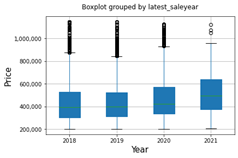
\includegraphics[width=0.5\linewidth]{fig1}
	\end{figure}
	
	
	Most samples are evenly distributed from 2018 - 2020 along with a few samples from 2021. When we show the 'price' in a boxplot with respect to year, we see that the range of price is significantly spread out. There are many points above maximum tail, which is a sign that our dataset may not be normally distributed with respect to each year. Further exploring the housing prices, we extracted the middle 90\% of the prices, yet there were still many outliers. However, we can see the mean price for 2018 - 2020 is around 400,000 while the mean price of 2021 is little bit higher. Because we only have few samples from 2021, we couldn't tell whether inflation impacts the 2021 prices.
	
	The main indicator of relevant data we used was correlation to the latestPrice attribute. When we created a correlation matrix of the integer values, we saw that numOfBathrooms field has the highest correlation with price of 0.5. For the Boolean values, we saw that none of these fields were particularly noteworthy, with hasSpa having the highest correlation of 0.17.
	
	\begin{figure}[H]
		\label{fig:fig2}
		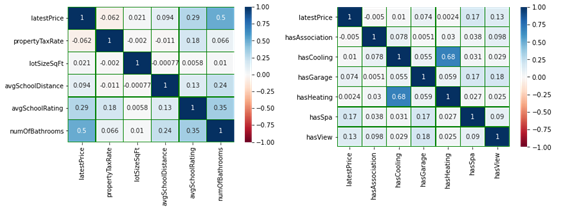
\includegraphics[width=1\linewidth]{fig2}
	\end{figure}
	
	For the floating-point values, we observed that livingAreaSqFt has the highest correlation of 0.47. The other closest correlations are 0.3 for numOfBedrooms, -0.2 for numOfHighSchools, and 0.2 for medianStudentPerTeacher. The zipcode and hometype categorical attributes were determined to not have relevant correlation with the price, so they were ignored.
	
	\begin{figure}[H]
		\label{fig:fig3}
		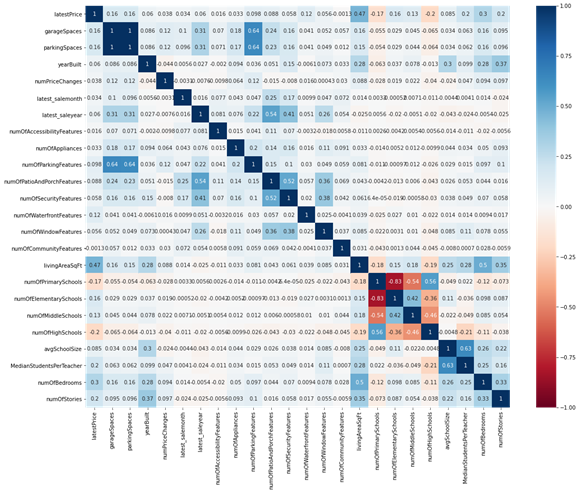
\includegraphics[width=1\linewidth]{fig3}
	\end{figure}
	
	\section{Proposed Methodology and Data Pre-processing}
	
	Since our goal is to predict the housing price, we decided to use Simple Linear Regression, Multiple Linear Regression, Polynomial regression, and Artificial Neural Network (ANN) for this numerical response variables. For regression methods, the output should be continuous numerical values. We figured that regression was the right methodology for our problem statement, considering that the dataset uses continuous values that we would be unsurprised to see fit a linear or polynomial regression model. In regression training processes (both linear and polynomial), we did not scale the data except for y data to make MSE values more easily comparable between models. For our application, we kept y values unscaled in regression so that the user could see a human-readable price prediction.
	
	We wanted to see if a neural network could compare, however, so we planned to work on a neural network model once the regression models were finished. For the ANN model, we divided the price to several ranges of intervals to make them classification problems with meaningful predictions. In ANN training processes, scaling data is required because each neuron receives inputs from all attributes. We used a MinMaxScaler to normalize our data to value between [0,1]. Also, since the response variable latestPrice is a numerical continuous variable, this implies that we could have at most N number of different prices as N is the number of samples in the dataset. This will make ANN hard to make useful in prediction on such huge amount of numerical price. Therefor we divided the price into several range of intervals of every \$50,000 from [0 – 600,000), every \$100,000 from [600,000 – 1,000,000), \$500,000 from [1,000,000 – 2,000,000), every \$1,000,000 from [2,000,000 – 10,000,000), and then all that were above \$10,000,000 were all in one price bucket. With limited numbers of price ranges as output, the ANN models can predict, with certain values of input attributes, which price range the data point should fall into.
	
	When determining which features to use, we considered the information gained from the exploratory analysis section, which revealed that numOfBathrooms, livingAreaSqFt, numOfBedrooms, avgSchoolRating, MedianStudentsPerTeacher, and numOfHighSchools all had the highest correlation for latestPrice. We saw that number of stories also had high correlation, but we did not include that one. It likely would have contributed mostly to similar information that the numOfBathrooms and numOfBedrooms explained. If we were to have done principle component analysis (PCA), we would likely have included it since the PCA would have handled features that were too similar for us.
	
	The simple linear regression had two options for highest correlating attributes: livingAreaSqFt and numOfBathrooms. However, even though numOfBathrooms had slightly higher correlation, it had a narrower set of options (1,2, etc.) that did not have the level of detail that livingAreaSqFt since it has much higher numbers. Therefore, our simple linear regression used livingAreaSqFt. The multiple linear regression, polynomial regression, and the artificial neural network used all of the viable options of features.
	
	\section{Experimental Results}
	
	\subsection{Simple Linear Regression}
	
	The simple linear regression measures the correlation between the living area square footage and the latest price of the house. According to the linear regression model, the testing MSE was 0.0031034538994231665, while the training MSE was 0.0007533569972620845. Since the testing MSE was much higher than the training MSE, it can be concluded that the simple linear regression showed signs of overfitting. Note that all of the above assumes the outliers have not been removed. When the outliers were removed, the training and testing MSEs are 0.01683046917734069 and 0.017602933835473195, respectively. The regression model no longer shows signs of overfitting but appeared to be much less accurate.
	
	
	\subsection{Multiple Linear Regression}
	
	The multiple linear regression uses the living area square footage, the number of bathrooms, the average school rating, the number of bedrooms, the number of high schools, and the median number of students per teacher, as the dependent variables. Just like before, the dependent variable is the latest price of the house. Assuming the outliers have not been removed, the training and testing MSEs turned out to be 0.001161543841697301 and 0.0026126372082117054, which indicates that the model shows signs of overfitting. Once the outliers have been removed, the training and testing MSEs became 0.015228611447641035 and 0.016849382441537858, respectively. Just like the simple linear regression model, the multiple linear regression model no longer shows signs of overfitting. The multiple linear regression model seemed to be more accurate than the simple linear regression model, although it remained relatively inaccurate.
	
	\subsection{Polynomial Regression}
	
	The polynomial regression uses the living area square footage, the number of bathrooms, the average school rating, the number of bedrooms, the number of high schools, and the median number of students per teacher, as the dependent variables. Just like before, the dependent variable is the latest price of the house. The data for the polynomial regression is shown below:
	
	\begin{figure}[H]
		\label{fig:fig4}
		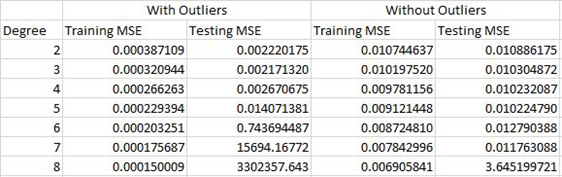
\includegraphics[width=1\linewidth]{fig4}
	\end{figure}
	
	When the outliers are present, the 3rd-degree polynomial regression appeared to be the most accurate model out of all the polynomial models that were created, with a training MSE of 0.000320944 and a testing MSE of 0.002171320. After the outliers are removed, however, the best polynomial regression model turned out to be the 5th-degree polynomial model, with a training MSE of 0.009121448 and a testing MSE of 0.010224790. Furthermore, the regression model no longer shows signs of overfitting once the outliers have been removed. The 5th-degree polynomial regression model appears to be more accurate than the simple and multiple linear regression models since it has a lower training and testing MSE than the linear regression models once the outliers have been removed.
	
	
	\subsection{Artificial Neural Network}
	
	The artificial neural network uses the living area square footage, the number of bathrooms, the average school rating, the number of bedrooms, the number of high schools, and the median number of students per teacher, as the dependent variables. Just like before, the dependent variable is the latest price of the house. The prices themselves have been divided into 22 different ranges. The ANN itself is based off Keras' sequential model and three hidden dense layers with 100, 80, and 50 nodes and ReLu as their activation functions while the output layer uses the sigmoid function. It uses stochastic-gradient descent as its optimizer and categorical\_crossentropy as its loss function. The output layer had 17 nodes since there were 17 different price bucket classes. Unfortunately, it ended up having an accuracy of .26, roughly, which was very undesirable. We tried to make the model more accurate by making the ANN more complex, less complex, and increasing epochs, but those options either led to overfitting or underfitting which reduced our accuracy even further. After exhausting those options, the conclusion was that the ANN was simply not viable for the predictions we were attempting. Perhaps it was the amount of price buckets that we used or the features that we chose that made it very incompatible with our data, but our focus was mainly on the regression models anyway.
	
	\subsection{Overall Results}
	
	\begin{figure}[H]
		\label{fig:fig5}
		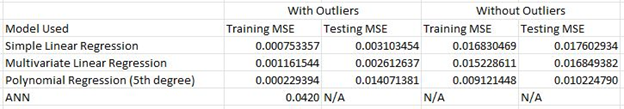
\includegraphics[width=1\linewidth]{fig5}
	\end{figure}

	Overall, it seemed that the 5th-degree polynomial degression was the most effective model at measuring the correlation between the price of the house and the other independent variables, especially if the outliers are removed. The linear regression models proved less effective than the 5th-degree polynomial regression model, but still had acceptably low training and testing MSEs. Without outliers removed, the multiple linear regression had the best performance.
	
	\subsection{Error Analysis}
	
	One possible reason why the models were not as accurate as they could be is the fact that too many samples have been removed from the dataset during preprocessing. Removing too many samples reduced the sample size, which made it more difficult to properly train models. The accuracy of these models suffered as a result. Keep in mind that removing outliers from the dataset is supposed to increase the accuracy of the models, not decrease it. The fact that removing the outliers decreased the accuracy of these models indicates that too many legitimate samples have been removed from the dataset. A post-experimental analysis of the regression models showed that the percentages of samples that were removed from the dataset was 3.72\% for simple linear regression (threshold = 2), 17.26\% for multiple linear regression (threshold = 2), and 11.28\% for polynomial regression (threshold = 3). The number of actual outliers could be counted with one or two hands with the help of a scatter plot. This means most of the samples removed during preprocessing were not true outliers. To remedy this, the threshold used to remove the outliers needs to be increased so that fewer legitimate samples would be removed from the dataset. Alternately, a manual effort to remove outliers would have probably been more efficient. For now, we will simply refer to the models where outliers were not removed to be our main output of this project. 
	
	\section{Conclusions and Discussion}
	
	This has yet to be written.
	
	\section{Sources}
	
	\begin{itemize}
		\item Abidoye, Rotimi Boluwatife, et al. “Predicting Property Price Index Using Artificial Intelligence Techniques.” International Journal of Housing Markets and Analysis, vol. 12, no. 6, Emerald Publishing Limited, 2019, pp. 1072–92, \url{https://doi.org/10.1108/IJHMA-11-2018-0095}.
		
		\item Kalliola, Jussiet et al. "Neural Network Hyperparameter Optimization for Prediction of Real Estate Prices in Helsinki." PeerJ Computer Science, 2021. ProQuest, https://www.proquest.com/scholarly-journals/neural-network-hyperparameter-optimization/docview/2514869195/se-2, doi:\url{http://dx.doi.org/10.7717/peerj-cs.444}.
		
		\item Mangaleswaran, Shivani and Vigneshwari S. “Prediction of Housing Prices Using Machine Learning, Time Series ARIMA Model and Artificial Neural Network.” ICDSMLA 2019 : Proceedings of the 1st International Conference on Data Science, Machine Learning and Applications, vol. 601, Springer, 2020, pp. 1002–08, \url{https://doi.org/10.1007/978-981-15-1420-3_110}.	
			
		\item Mu, Jingyi et al. "Housing Value Forecasting Based on Machine Learning Methods", Abstract and Applied Analysis, vol. 2014, Article ID 648047, 7 pages, 2014. \url{https://doi.org/10.1155/2014/648047}.
		
		\item Park, Byeonghwa, and Jae Kwon Bae. “Using Machine Learning Algorithms for Housing Price Prediction: The Case of Fairfax County, Virginia Housing Data.” Expert Systems with Applications, vol. 42, no. 6, Elsevier Ltd, 2015, pp. 2928–34, \url{https://doi.org/10.1016/j.eswa.2014.11.040}.
		
		\item Selim, Hasan. “Determinants of House Prices in Turkey: Hedonic Regression Versus Artificial Neural Network.” Expert Systems with Applications, vol. 36, no. 2, Elsevier Ltd, 2009, pp. 2843–52, \url{https://doi.org/10.1016/j.eswa.2008.01.044}.
	\end{itemize}

	\subsection{LaTeX Document Sources}

	\begin{itemize}
		\item Cocker, Aaron. "A introduction to creating documents in LaTeX." opensource.com. \url{https://opensource.com/article/17/6/introduction-latex}.
		\item "How to make clickable links in LaTeX." LaTeX-Tutorial.com. \url{https://latex-tutorial.com/tutorials/hyperlinks/}.
		\item "Insert an image in LaTeX - Adding a figure or picture." LaTeX-Tutorial.com. \url{https://latex-tutorial.com/tutorials/figures/}.
		\item "Lists." Overleaf. \url{https://www.overleaf.com/learn/latex/Lists}.
		
	\end{itemize}
		
\end{document}